\clearpage
\begin{figure*}[t]
    \centering
    \counterwithin{figure}{section}
    \renewcommand\thefigure{C\arabic{figure}}
    \begin{subfigure}[t]{0.69\linewidth}
    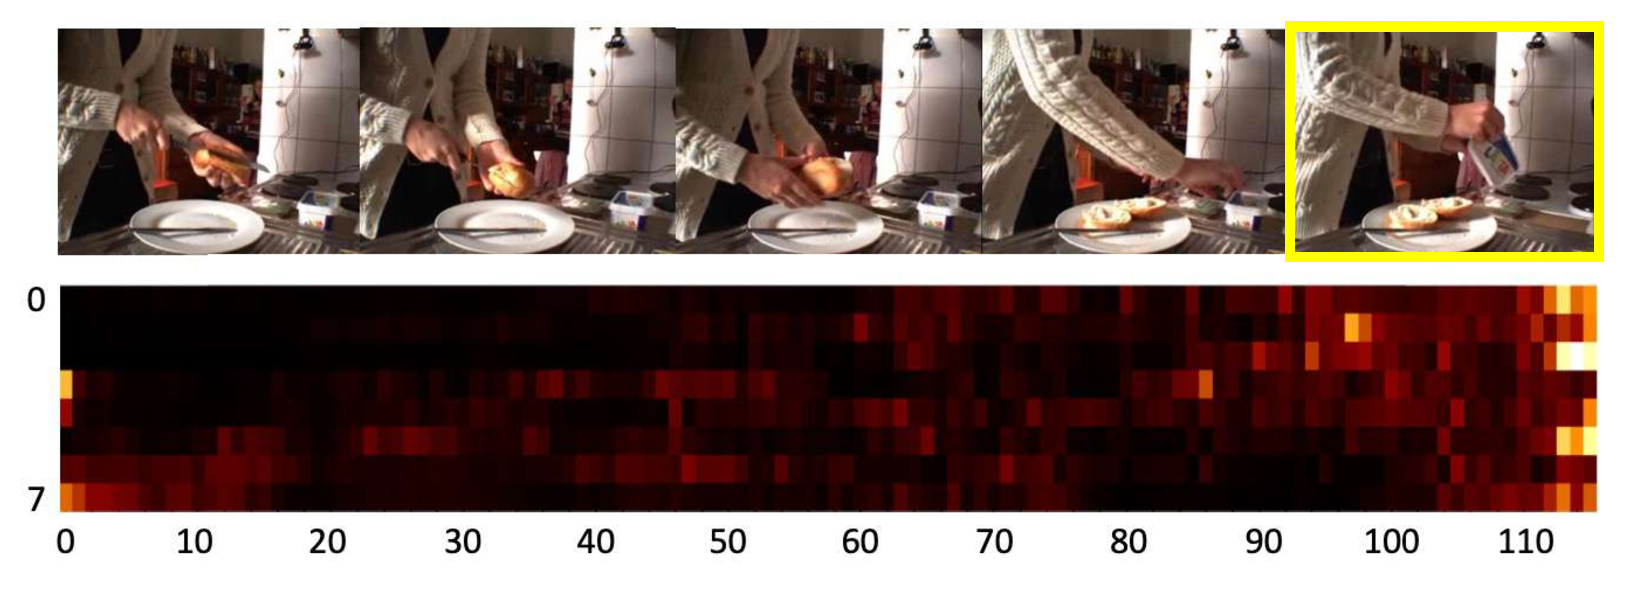
\includegraphics[width=\columnwidth]{Figures/pdf/sattn1_compressed.pdf}
    \counterwithin{figure}{section}
    \renewcommand\thefigure{S\arabic{figure}}
    \vspace{-5mm}
    \caption{Activity: Sandwich}
    \label{fig:s4a}
    \end{subfigure}
    
    \vspace{3mm}
    
    \begin{subfigure}[t]{0.75\linewidth}
    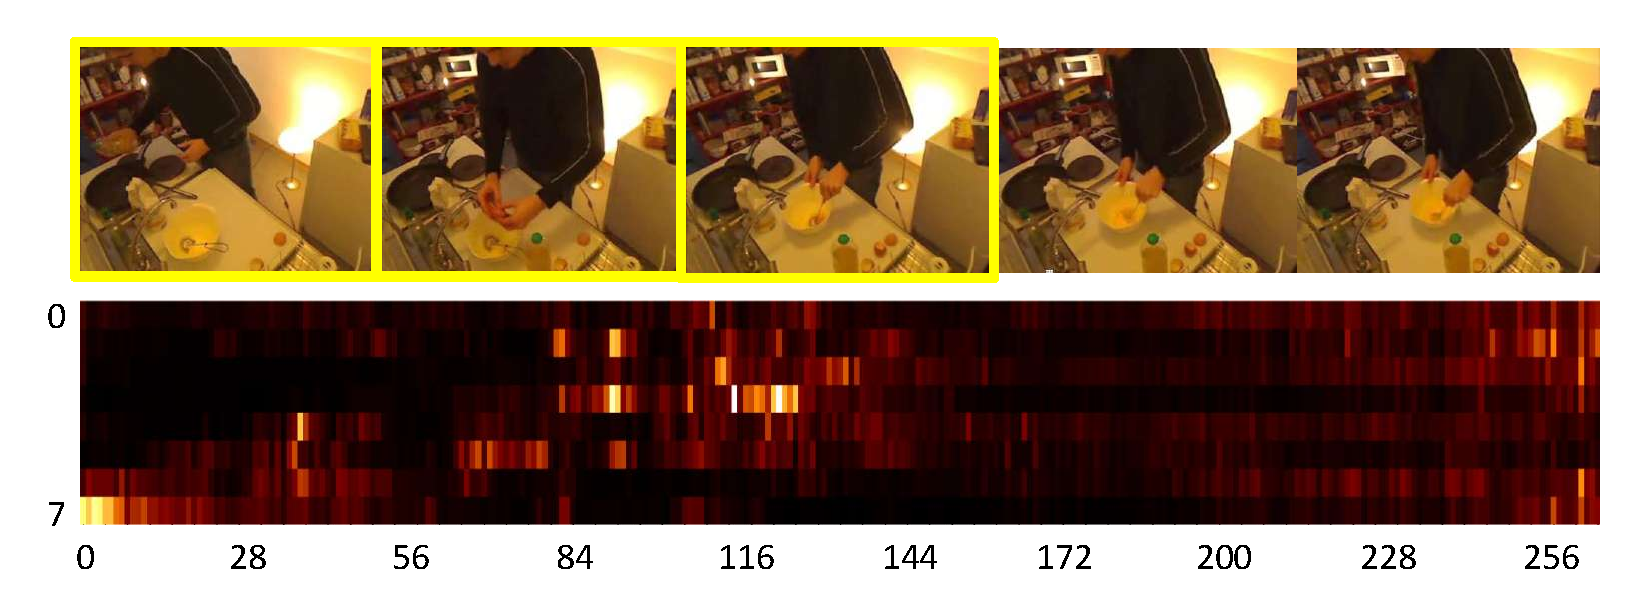
\includegraphics[width=\columnwidth]{Figures/pdf/sattn2_compressed.pdf}
    \counterwithin{figure}{section}
    \renewcommand\thefigure{S\arabic{figure}}
    \vspace{-6mm}
    \caption{Activity: Scramble egg}
    \label{fig:s4b}
    \end{subfigure}
    
    \vspace{3mm}
    
    \begin{subfigure}[t]{0.75\linewidth}
    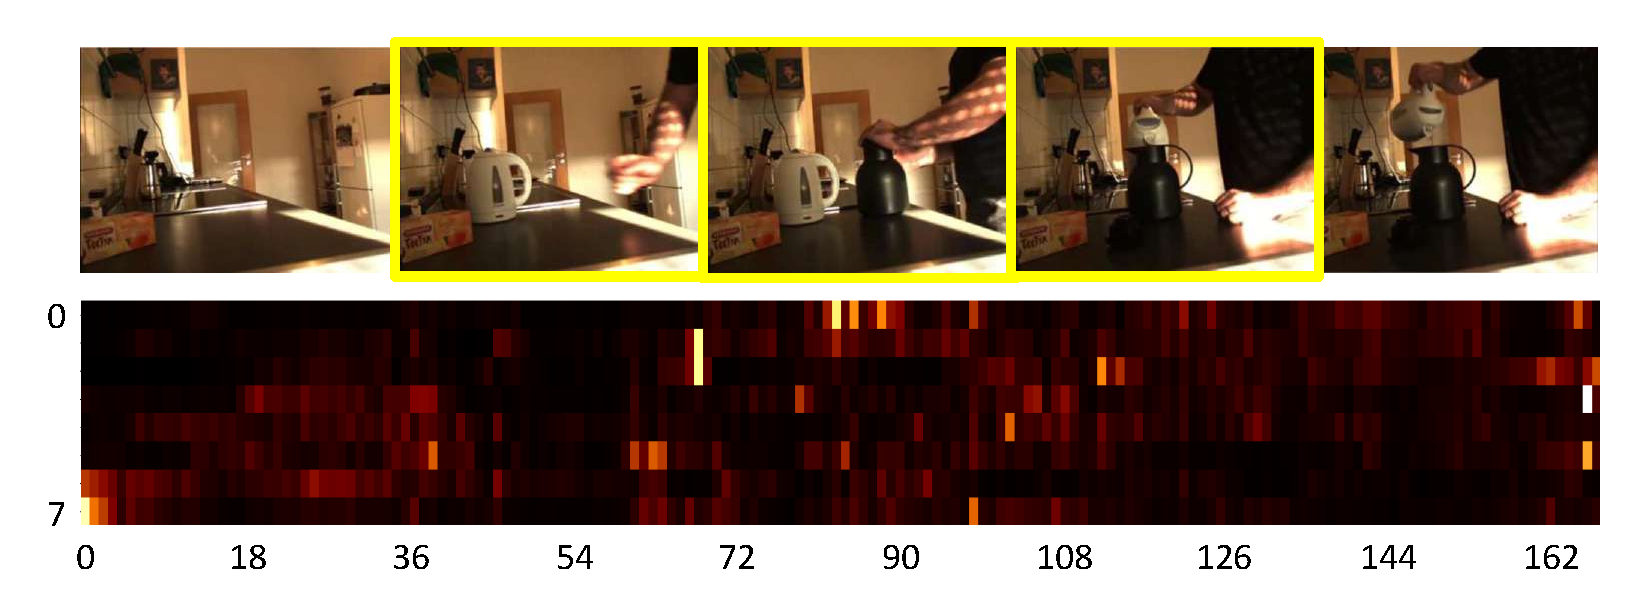
\includegraphics[width=\columnwidth]{Figures/pdf/sattn4_compressed.pdf}
    \counterwithin{figure}{section}
    \renewcommand\thefigure{S\arabic{figure}}
    \vspace{-6mm}
    \caption{Activity: Tea}
    \label{fig:s4d}
    \end{subfigure}
    
    \vspace{3mm}
    
    \begin{subfigure}[t]{0.75\linewidth}
    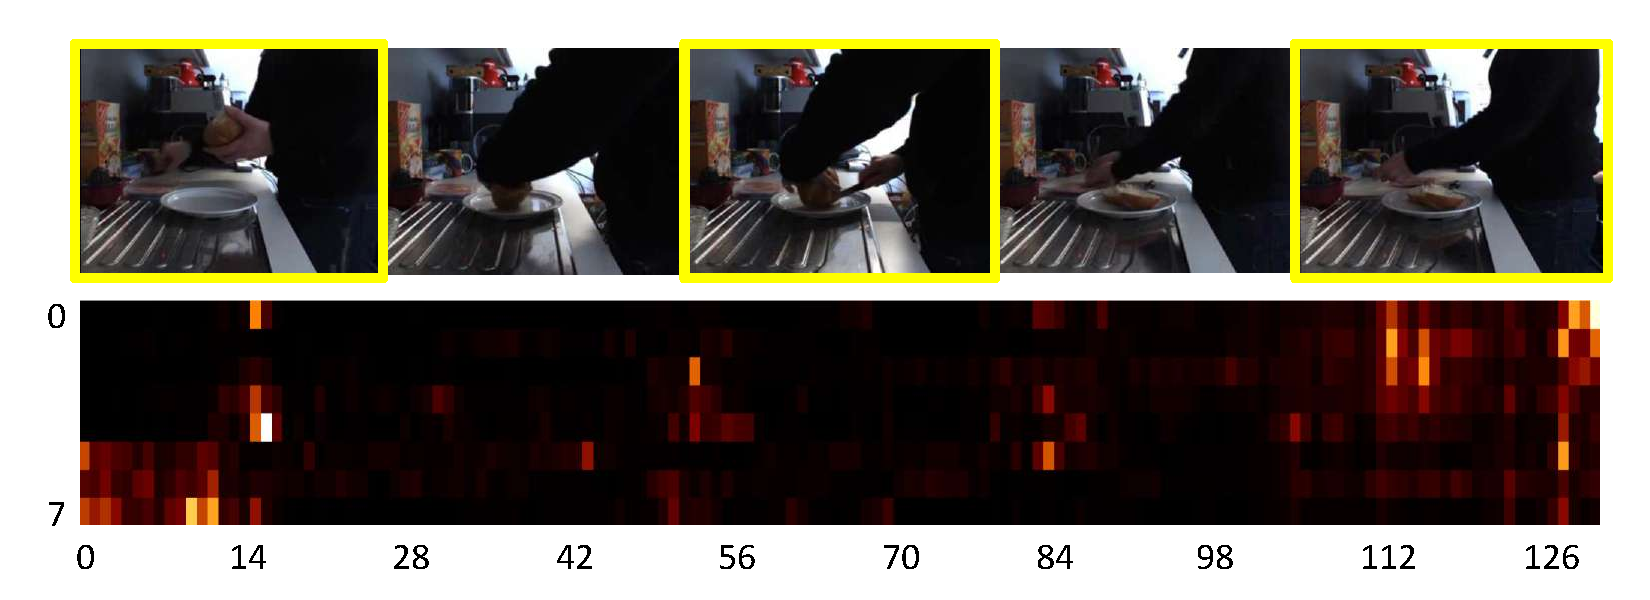
\includegraphics[width=\columnwidth]{Figures/pdf/sattn5_compressed.pdf}
    \counterwithin{figure}{section}
    \renewcommand\thefigure{S\arabic{figure}}
    \vspace{-6mm}
    \caption{Activity: Sandwich}
    \label{fig:s4e}
    \end{subfigure}
\counterwithin{figure}{section}
\renewcommand\thefigure{S\arabic{figure}}
\caption{\textbf{Cross-attention map visualization on Breakfast}. The vertical and horizontal axis indicates the decoder queries and observed frames, respectively. The brighter color indicates a higher attention score. RGB frames above the attention map are sampled uniformly from the video.
We emphasize the frames with high attention scores with yellow box and other frames are uniformly sampled. Best viewed in color.}
\vspace{-2mm}
 \label{fig:sup_attn}
\end{figure*}